\documentclass[
    paper=a4,               % paper format
    fontsize=10pt,          % fontsize
    %twoside,               % double-sided
    open=right,             % begin new chapter on right side
    titlepage=false,        % use no standard title page
    parskip=half,           % set paragraph skip to half of a line
]{scrreprt}                 % KOMA-script report

\raggedbottom{}

% Load Standard Packages:
%---------------------------------------------------------------------------
\usepackage{scrpage2}
\usepackage[standard-baselineskips]{cmbright}
\usepackage[ngerman]{babel}                                             % german hyphenation
\usepackage[utf8]{inputenc}                                             % UTF-8 character encoding
\usepackage[T1]{fontenc}                                                % hyphenation of words with ä,ö and ü
\usepackage{textcomp}                                                   % additional symbols
\usepackage{ae}                                                         % better resolution of Type1-Fonts 
\usepackage{etoolbox}                                                   % color manipulation of header and footer
\usepackage{graphicx}                                                   % integration of images
\usepackage{float}                                                      % floating objects
\usepackage{caption}                                                    % for captions of figures and tables
\usepackage{booktabs}                                                   % package for nicer tables
\usepackage{tocvsec2}                                                   % provides means of controlling the sectional numbering
\usepackage[square,sort,comma,numbers]{natbib}                          % provides various citation styles
\usepackage{wrapfig}                                                    % provides floating of text around images
\usepackage{nameref}                                                    % provides printing names of references
\usepackage{multicol}                                                   % Foo
\usepackage{subcaption}
%---------------------------------------------------------------------------

%---------------------------------------------------------------------------
% Set up page dimension
%---------------------------------------------------------------------------
\usepackage{geometry}
\geometry{a4paper,
    left=28mm,
    right=15mm,
    top=30mm,
    headheight=20mm,
    headsep=10mm,
    textheight=242mm,
    footskip=15mm
}
%---------------------------------------------------------------------------

\begin{document}

    \title{Semantische Datenbanken}

    Computer Perception and Virtual Reality / Prof.\ Dr.\ Jürgen Eckerle\\
    Experte: Jean-Marie Leclerc

    % Lead: 480
    \textbf{Der klassische Ansatz der Wissensabbildung, zum Beispiel in Form von UML, welchem die relationale Datenspeicherung zugrunde liegt, wird in der heutigen Informatik weitläufig eingesetzt und ist de facto Standard. Häufig geschieht dies in enger Verbindung mit der objektorientierten Programmierung. Experten aus einer Fachrichtung sind fähig diese Daten zu interpretieren und daraus Schlüsse zu ziehen. Es ist nicht möglich Fragestellungen zu beantworten, welche über reine Relationsverknüpfungen hinausgehen. Mit dieser Technik sind Objekteigenschaften und -Verhalten also eher schwer abbildbar. Eine andere Art Wissen zu repräsentieren sind semantische Datenbanken. Diese ermöglichen das Abbilden von Objekteigenschaften und -Verhalten und können mithilfe von Schlussfolgerungen die Rolle des Experten einnehmen.}

    % Text: 2400
    \begin{multicols}{3}
        \section*{Wissenabbildung}
        Semantische Datenbanken werden in so genannten Ontologien abgebildet. Diese werden überall dort verwendet, wo Semantik zur Formulierung von Informationen genutzt wird. Eine Ontologie beschreibt Wissen rund um eine Wissens- bzw. Problemdomäne. Ontologien werden in Form von Tripeln abgelegt, wobei die Tripel die Form \textit{Subjekt Prädikat Objekt} haben. Also zum Beispiel \textit{Seilpark hatStandort Balmberg}. So können Objekte und deren Eigenschaften sowie Beziehungen zwischen Objekten abgebildet werden.

        Eine weitere Komponente der Wissensabbildung ist die Verwendung von Regeln. Diese ermöglichen es Schlüsse zu ziehen, so kann zum Beispiel definiert werden, dass wenn ein Reise Mut erfordert diese actionreich ist.
        
        Aufgrund einer Wissensbasis, bestehend aus einer Ontologie und Regeln, können mithilfe eines Reasoners (Inferenz-Maschine) Schlüsse gezogen werden.
        Ein Reasoner ist eine Software-Komponente, welche mithilfe von Inferenz und Resolution zusätzliches Wissen ableiten kann. Dazu wird Beschreibungslogik (welche Teil der Prädikatenlogik ist) genutzt.

        \section*{Aufgabenstellung und Umsetzung}
        Ziel dieser Arbeit ist der Aufbau einer semantischen Datenbank, anhand einer konkreten Wissensdomäne, sowie der Nutzung der Datenbank. Weiter soll gezeigt werden, wie ein Knowledge Engineer bei der Wissensmodellierung, in Form von Ontologien, vorgeht.

        Konkret wurde die Wissensdomäne Reiseplanung gewählt, denn in der heutigen Zeit werden Ferien häufig per Internet gebucht. Was aber, wenn der Urlaub nicht einfach zwei Wochen an einem Ort stattfinden soll? Was, wenn der Kunde reisen möchte? Oder sonstige spezielle Wünsche hat? Für solche Anforderungen muss er auch heute noch in ein Reisebüro um sich beraten zu lassen.

        Damit dieses Ziel erreicht werden konnte, wurde zuerst eine Ontologie in Form von Klassen, Individuen, Relationen und Eigenschaften erstellt. Da dies jedoch schnell ins Uferlose übergehen kann, wenn kein klarer Rahmen definiert ist, wurde die Ontologie, anhand exemplarischer Reisen schrittweise aufgebaut.

        Normalerweise werden Abfragen in einer Ontologie mittels einer Abfragesprache getätigt. Diese benötigt jedoch viel Fachwissen und Wissen über den Aufbau einer Ontologie. Um dennoch eine benutzerfreundliche Reiseplanung zu bieten, wurde eine Webapplikation zur Reiseplanung entwickelt. Diese ermöglicht das Planen einer Reise mithilfe eines Assistenten. Der Benutzer kann die gewünschten Reisekriterien auswählen. Er erhält als Ergebnis eine Auswahl an Objekten, welche seinen gewählten Kriterien entsprechen.

        Der theoretische Teil der Arbeit wurde in Form eines Dokumentes mit tutorialcharakter erstellt. Dieses zeigt das Vorgehen zum Aufbau und zur Nutzung eines Expertensystems schrittweise auf.

    \end{multicols}

    % \begin{minipage}[hbt]{5cm}
    %     \centering
    %     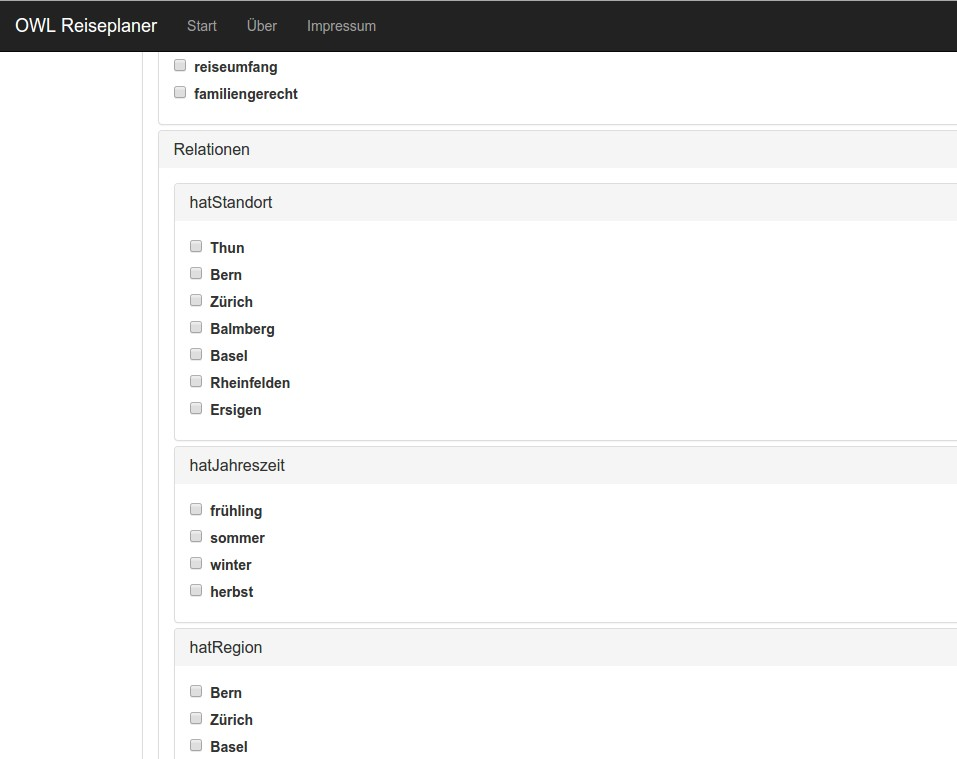
\includegraphics[width=5cm]{bilder/reiseplaner_gui.jpg}
    %     \captionof*{figure}{Benutzeroberfläche des Reiseplaners}
    % \end{minipage}
    % \hfill
    % \begin{minipage}[hbt]{5cm}
    %     \centering
    %     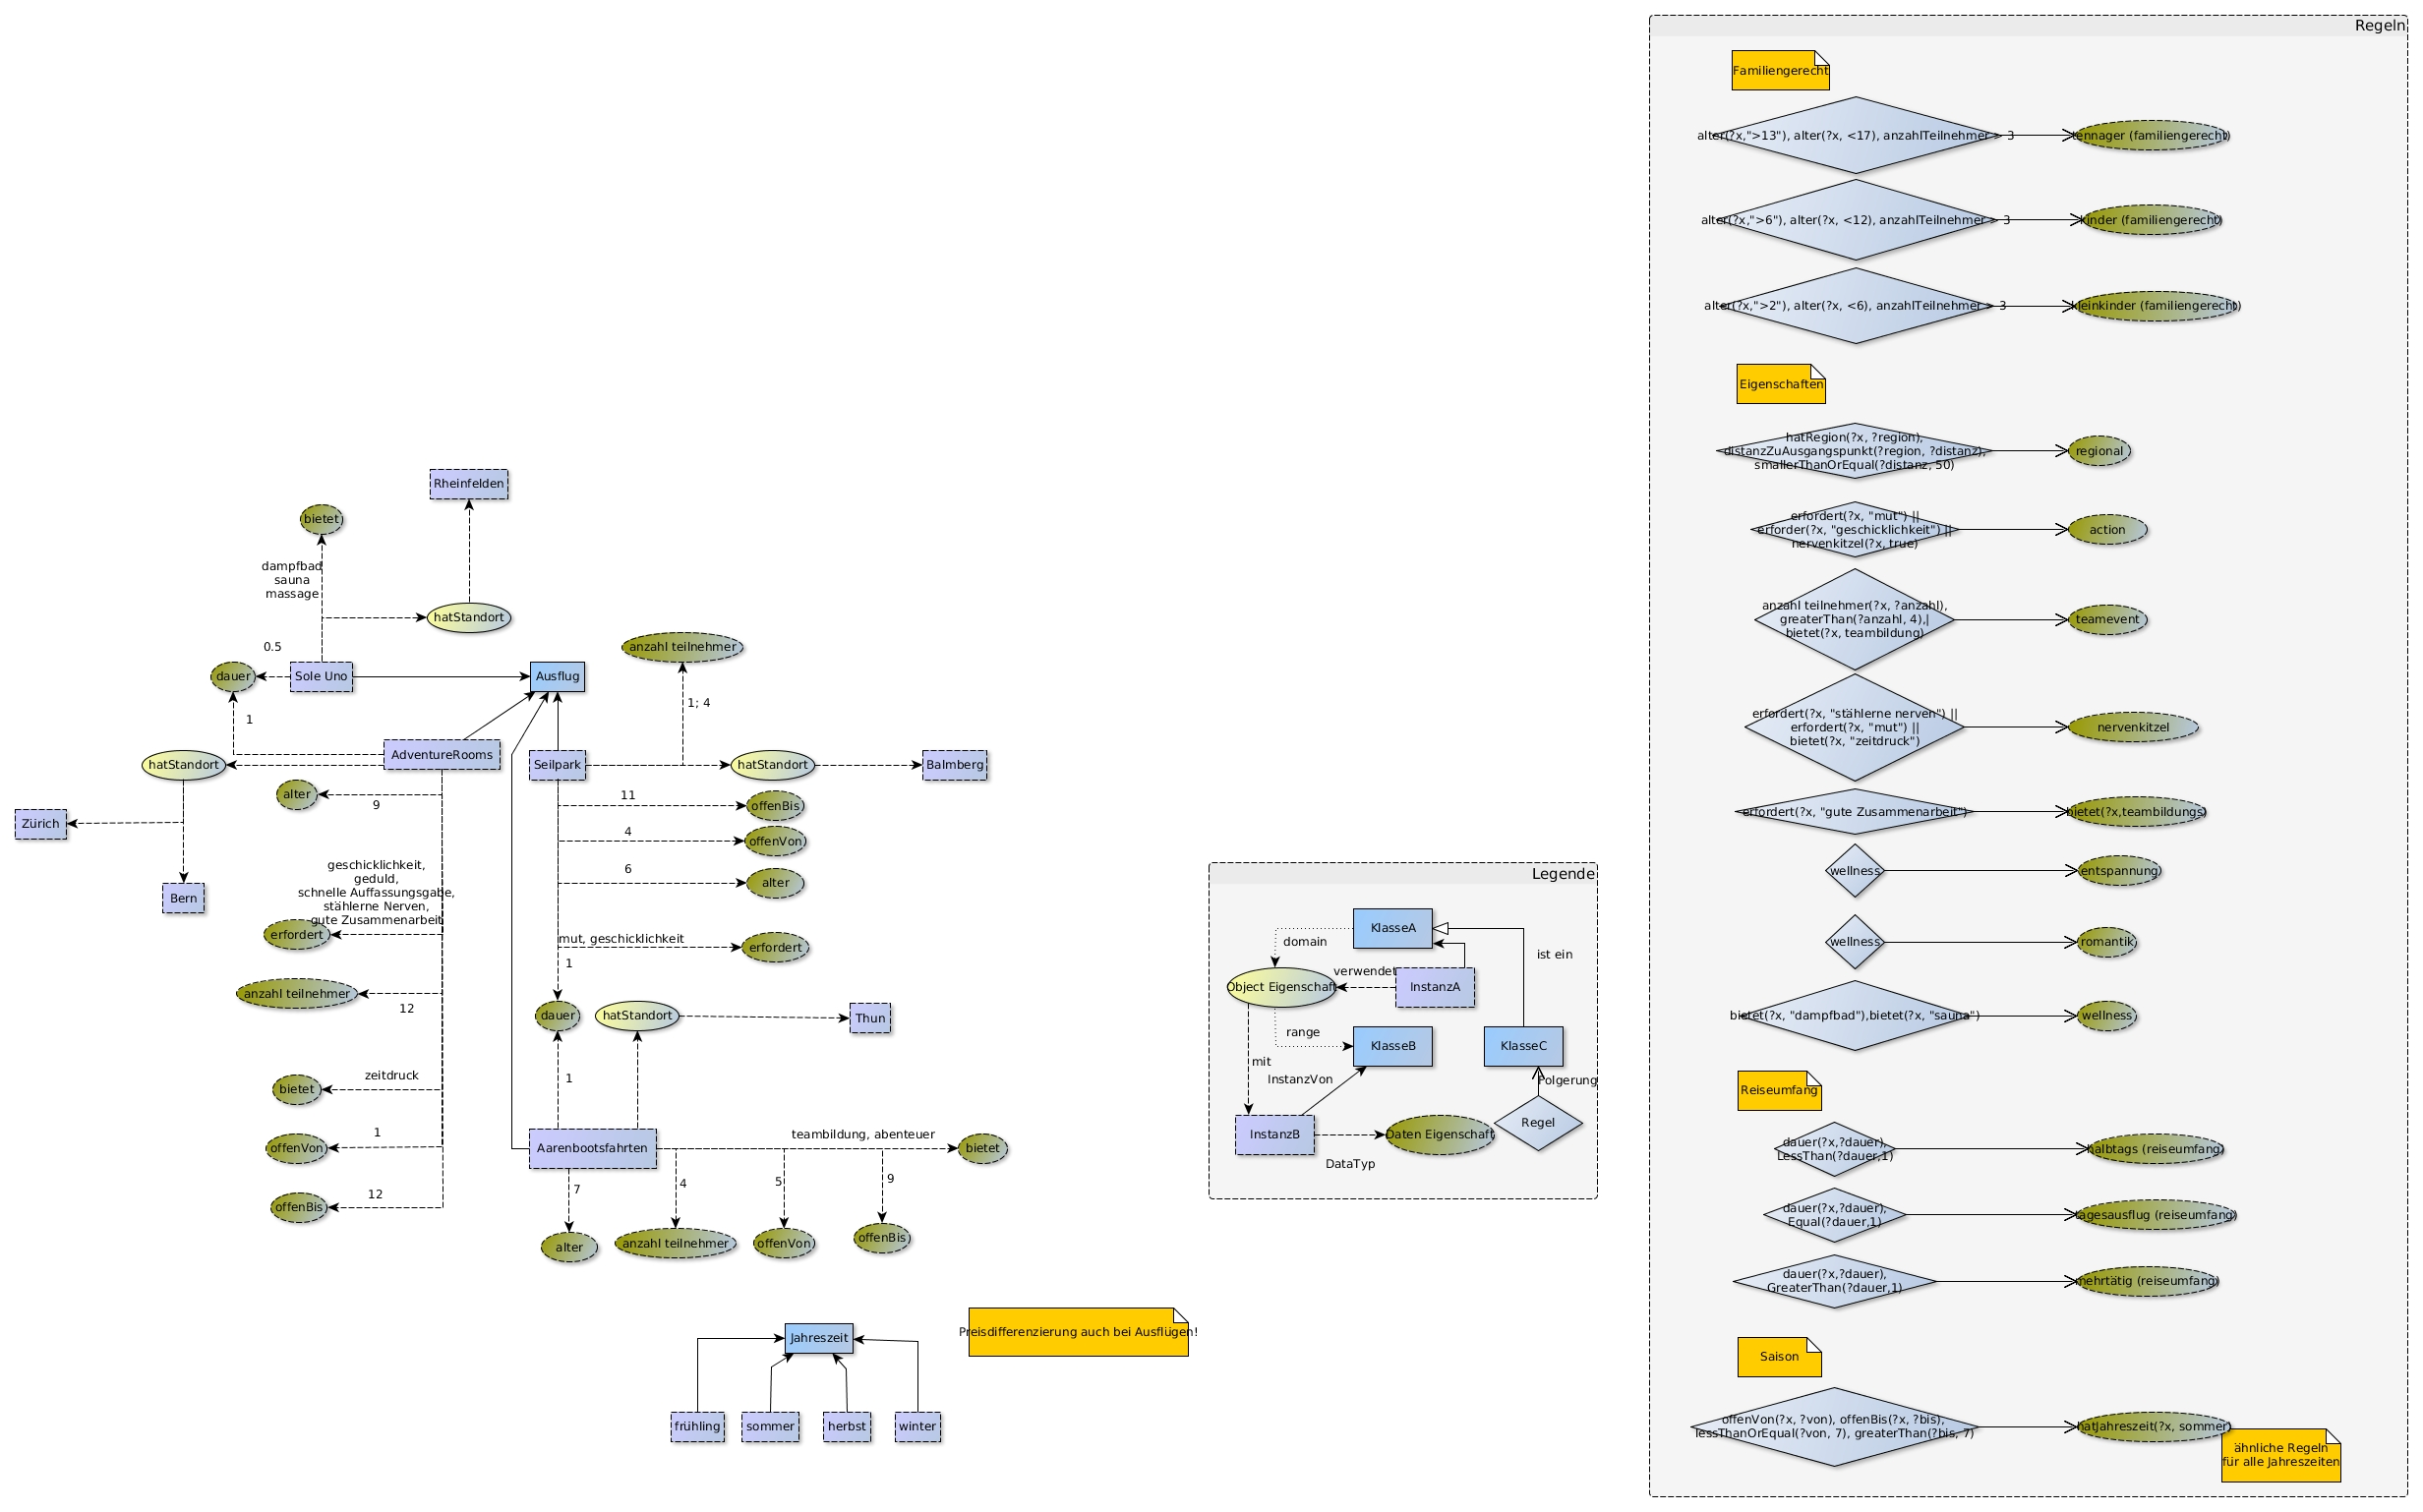
\includegraphics[width=5cm]{bilder/semantisches_netz.jpg}
    %     \captionof*{figure}{Semantisches Netz des Reiseplaners}
    % \end{minipage}

    % \begin{figure}[h]
    %     \begin{subfigure}{5cm}
    %         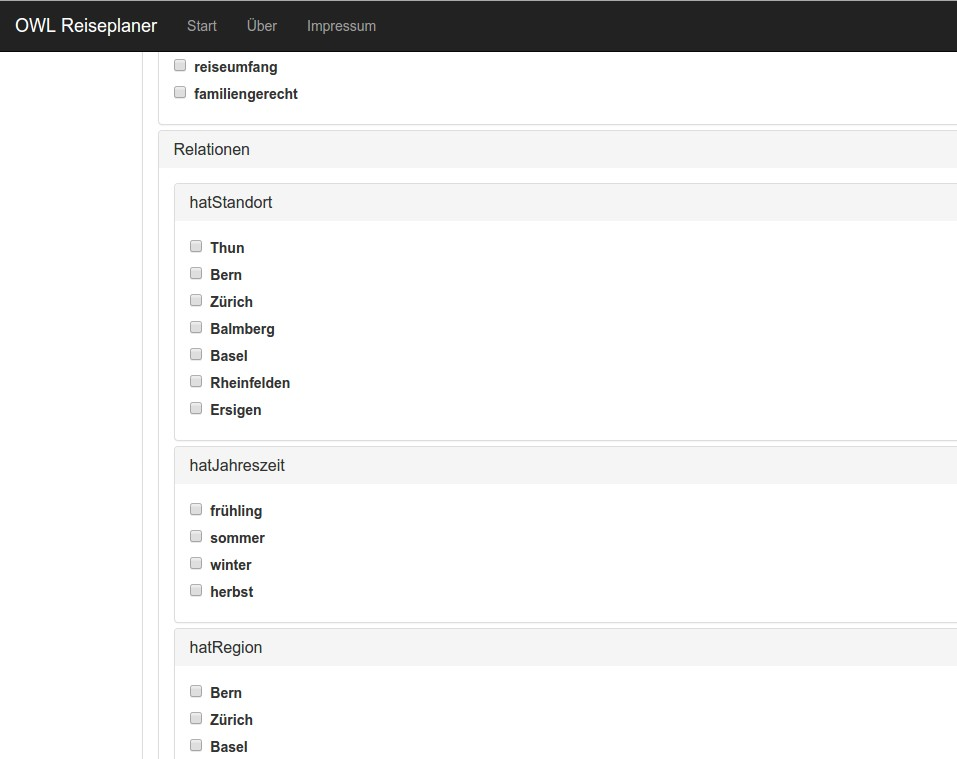
\includegraphics[scale=0.2]{bilder/reiseplaner_gui.jpg}
    %         \caption{horse}
    %         \label{fig:horse}
    %     \end{subfigure}
    %     \hspace{2cm}
    %     \begin{subfigure}{5cm}
    %         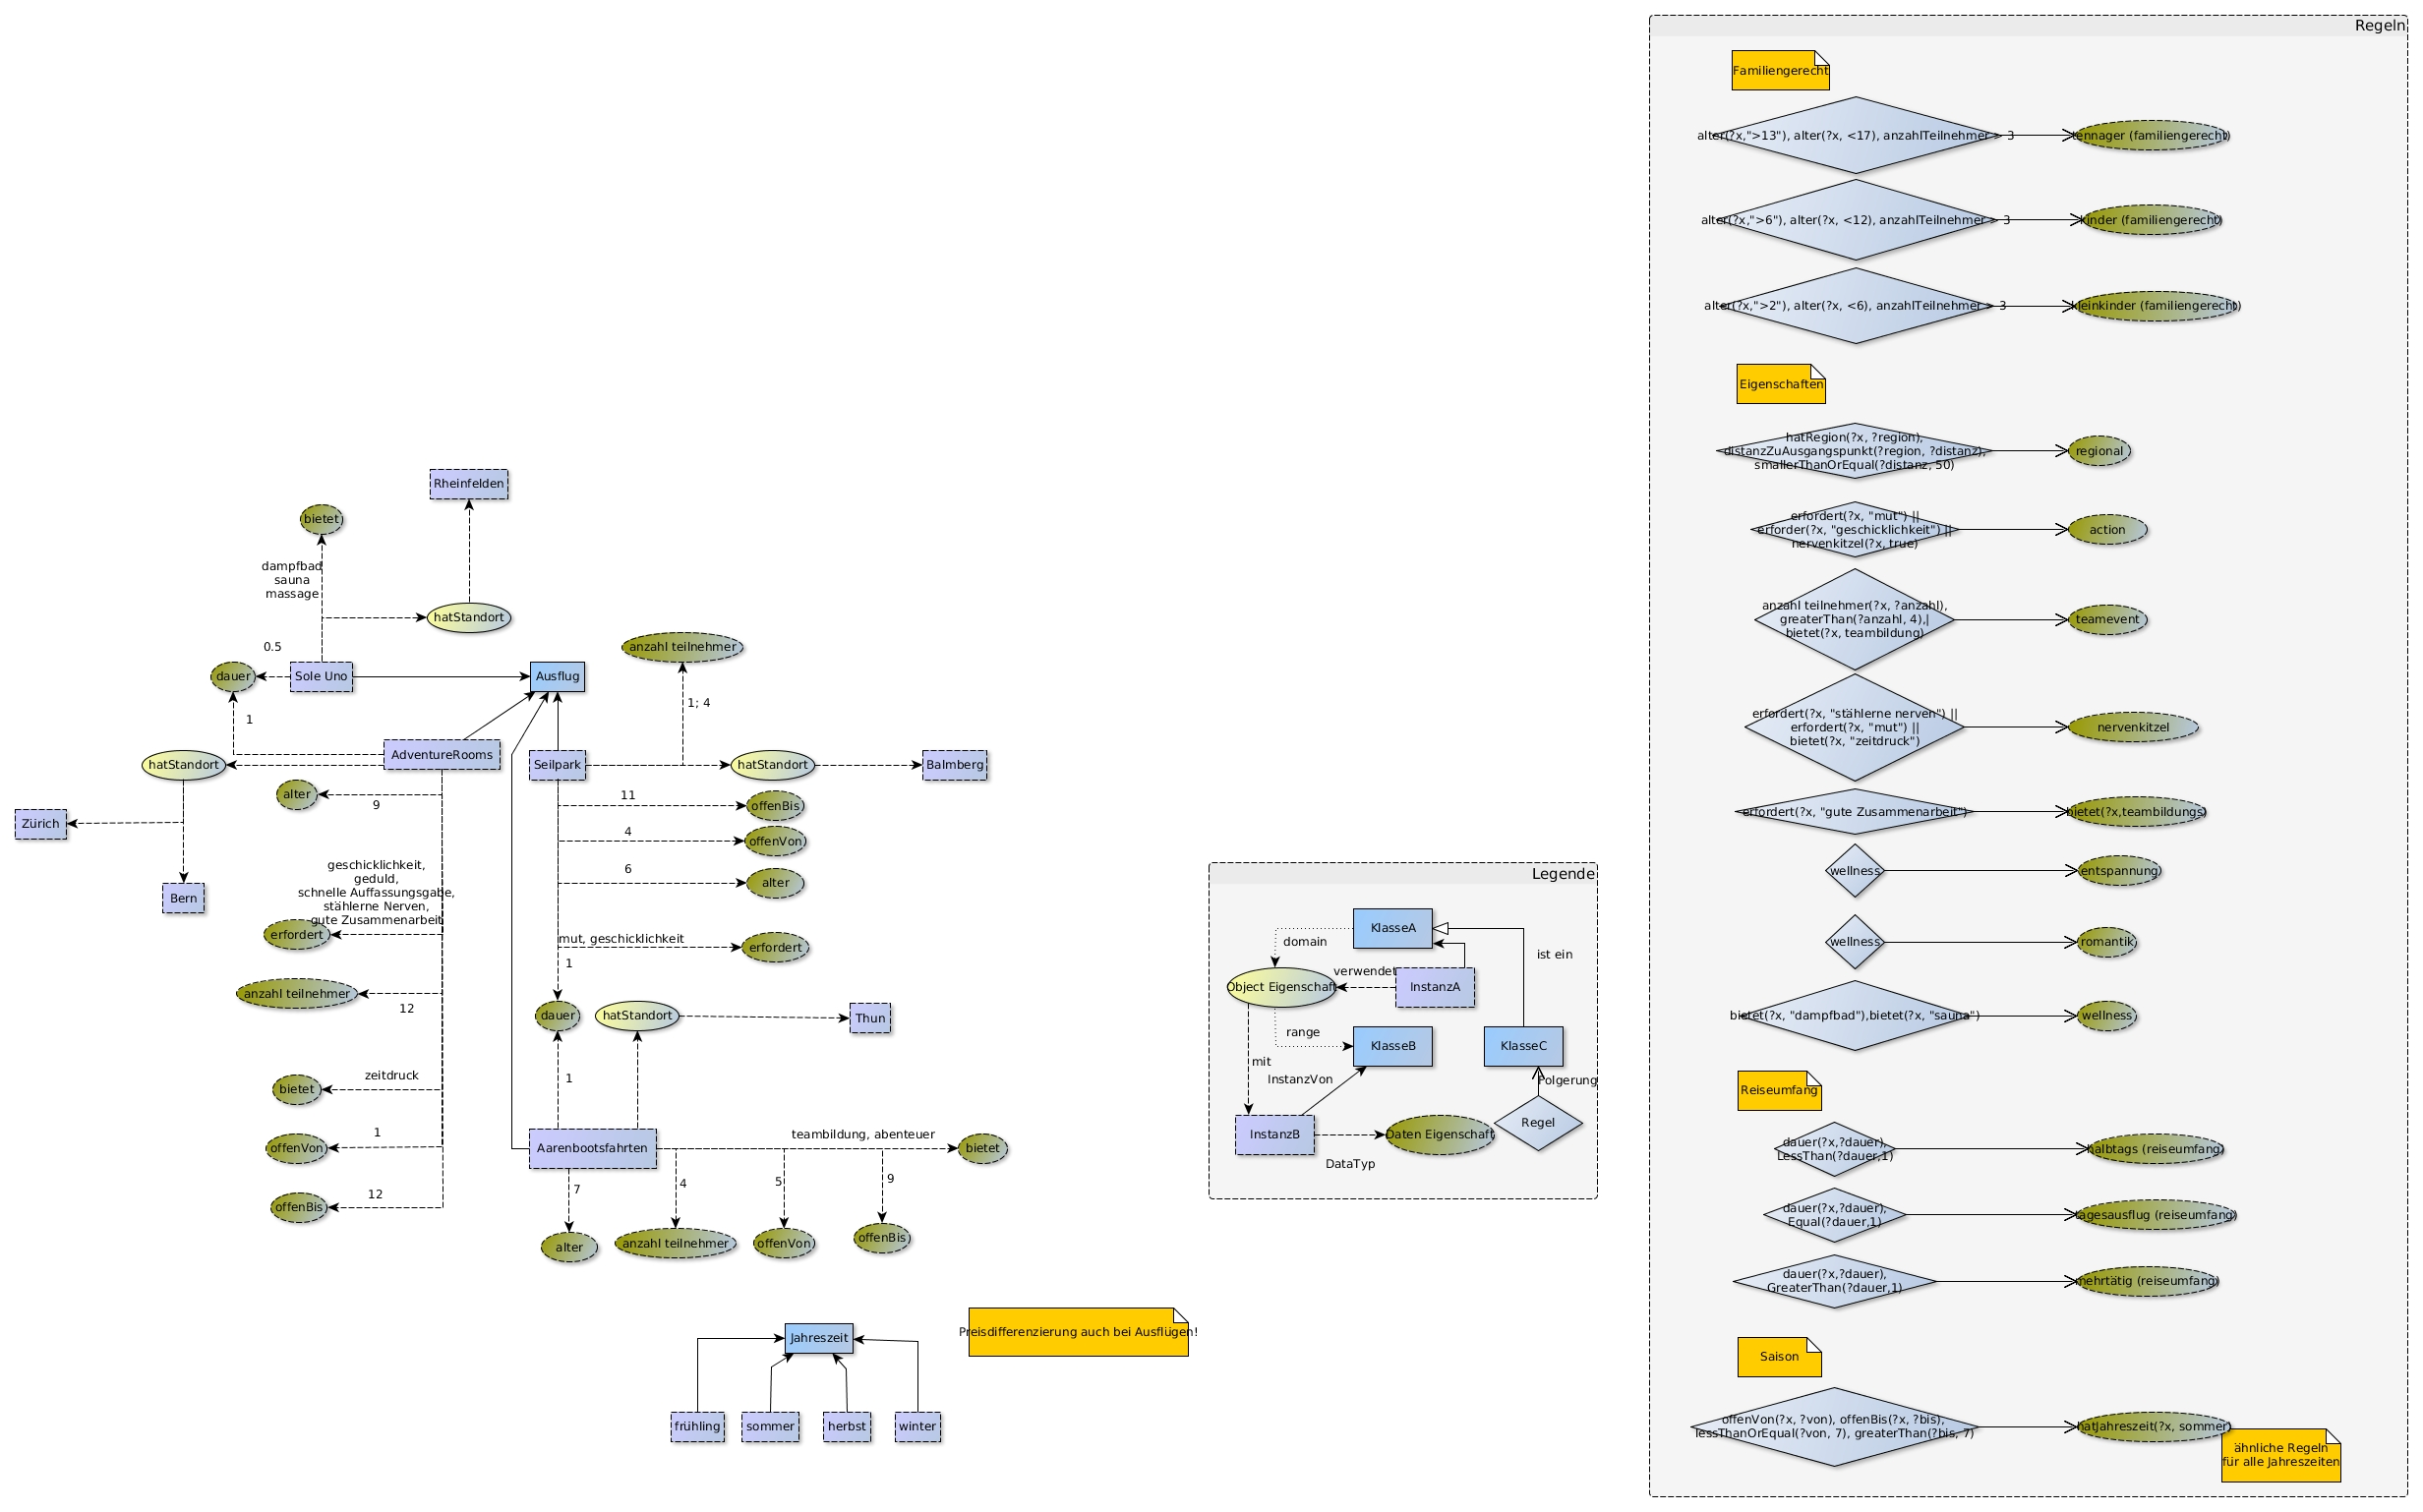
\includegraphics[scale=0.2]{bilder/semantisches_netz.jpg}
    %         \caption{zebra}
    %         \label{fig:zebra}
    %     \end{subfigure}
    %     \caption{animals}
    %     \label{fig:animals}
    % \end{figure}
    % Figure~\ref{fig:animals} shows some animals. Figure~\ref{fig:horse} shows a horse.
    \begin{figure}[htbp]
        \begin{minipage}[hbt]{0,49\textwidth}
            \centering
            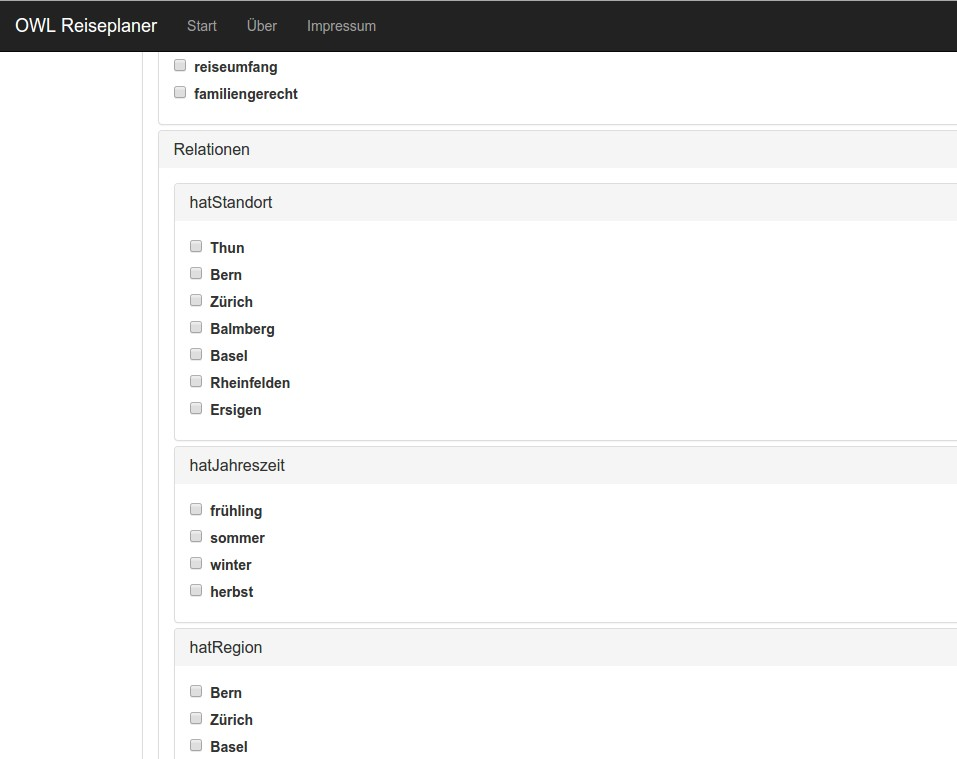
\includegraphics[scale=0.1]{bilder/reiseplaner_gui.jpg}
            \caption*{Benutzeroberfläche des Reiseplaners}
        \end{minipage}
        \begin{minipage}[hbt]{0,49\textwidth}
            \centering
            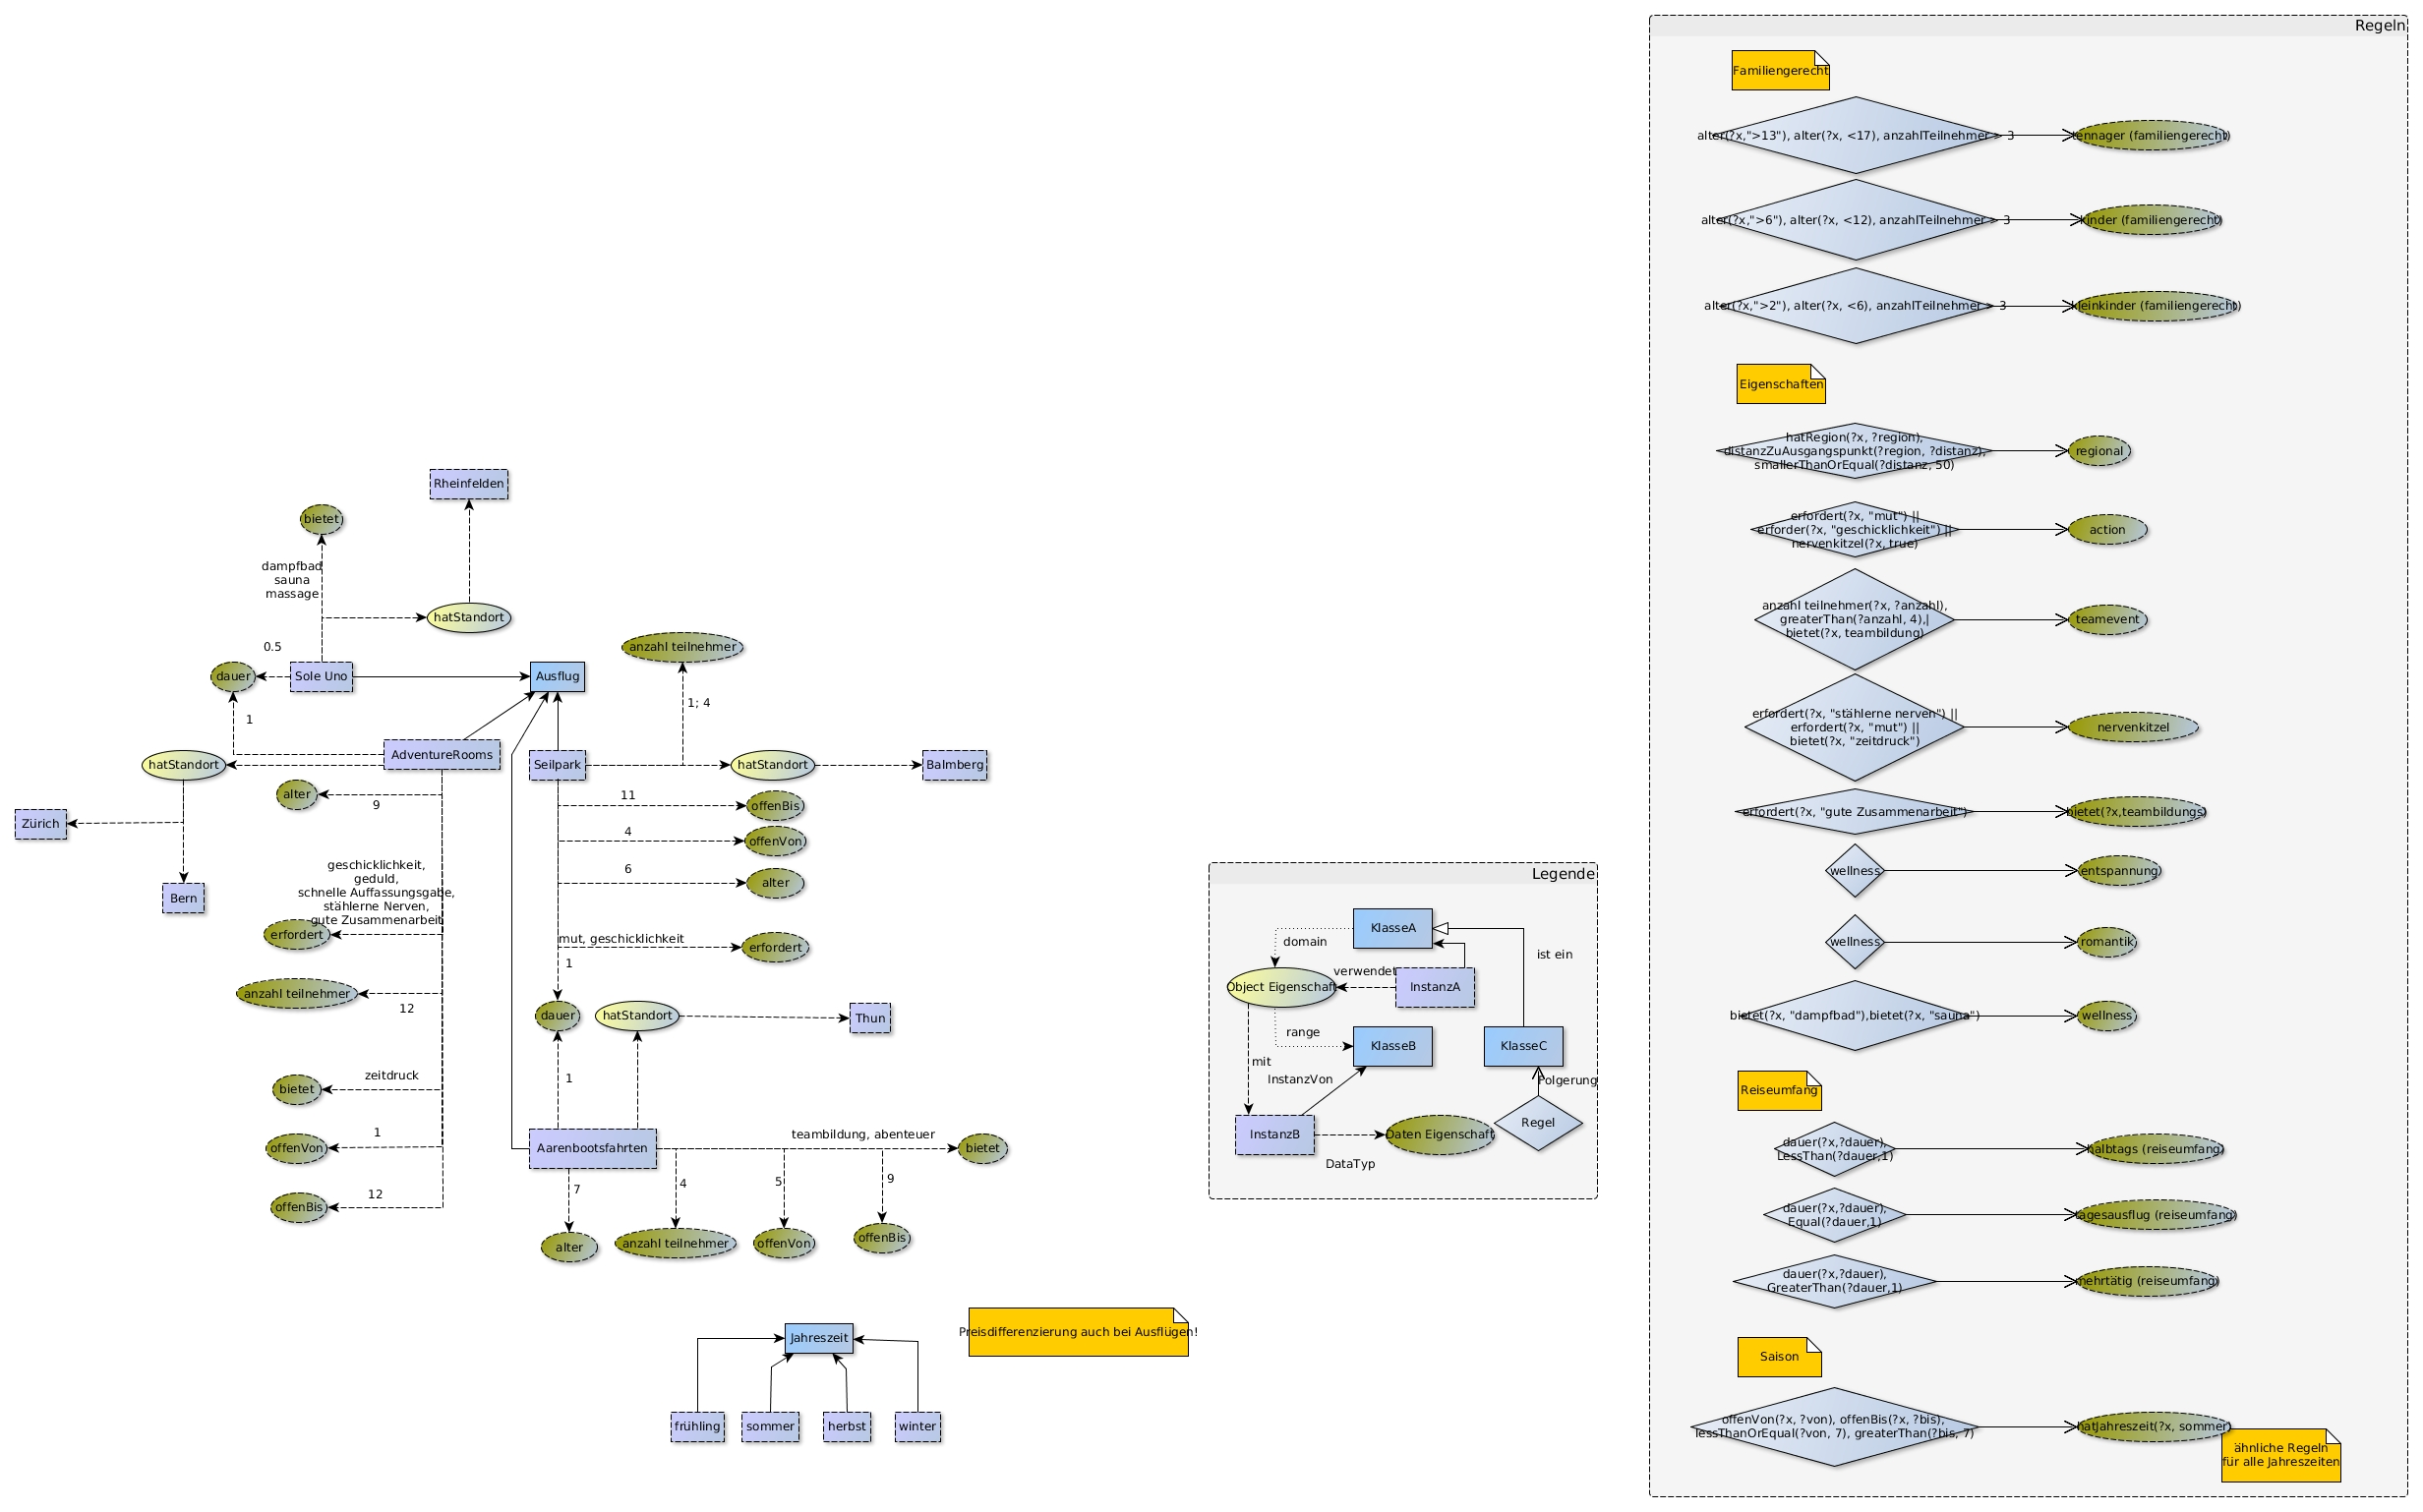
\includegraphics[scale=0.06]{bilder/semantisches_netz.jpg}
            \caption*{Reiseplaner als semantisches Netz}
        \end{minipage}
    \end{figure}
\end{document}
